\documentclass[11pt]{beamer}
\usepackage{
	xcolor,
	graphicx,
	subcaption,
	bm,
	pifont,
	booktabs,
	multirow,
	float,
	amsmath, 
	amssymb,
	appendixnumberbeamer
	} 
%\usefonttheme[onlymath]{serif} % mathmode font like in article TeX	

% https://tex.stackexchange.com/questions/565069/beamer-bold-math-no-longer-working
% allows for boldface in beamer
\DeclareFontShape{OT1}{cmss}{b}{n}{<->ssub * cmss/bx/n}{} 

	
\usetheme{Madrid}

\definecolor{emc-darkblue}{RGB}{14, 36, 112}
\definecolor{emc-lightblue}{RGB}{153, 209, 232}
\definecolor{ggray}{RGB}{208, 208, 208}


\setbeamercolor{palette primary}{bg=emc-darkblue, fg=white}
\setbeamercolor{palette secondary}{bg=emc-lightblue, fg=emc-darkblue}
\setbeamercolor{palette tertiary}{bg=emc-darkblue, fg=white}
\setbeamercolor{structure}{fg=emc-darkblue} 
\setbeamercolor{section in toc}{fg=emc-darkblue} 

\title[CITRUS]{Convergence for Individualizing TReatment Using Statistical approaches (CITRUS)}


\author[Welz, ten Haaf, Alfons]{\underline{Max Welz}\inst{1,2} \and Kevin ten Haaf\inst{2} \and Andreas Alfons\inst{1}}
\institute[]{\inst{1} Erasmus University Rotterdam, Dept. of Econometrics \and \inst{2} Erasmus Medical Center, Dept. of Public Health}

\titlegraphic{
\includegraphics[width=5cm]{eur-logo.png}}

\date[October 21, 2021]{October 21, 2021 \\\bigskip TI PhD Seminar}

\pgfdeclareimage[height=0.5cm]{university-logo}{eur-stamp.png}
\logo{\pgfuseimage{university-logo}}


% Delete this, if you do not want the table of contents to pop up at
% the beginning of each section:



%%%%%%%%% bugfix for TeXShop:
\makeatletter
\let\@@magyar@captionfix\relax
\makeatother



%%%%%%%% Bibliography
% capitalization of Dutch names (function applicable to bib file)
\DeclareRobustCommand{\VAN}[3]{#3}

 
%%  bib settings
\usepackage{natbib}
\setcitestyle{authoryear} 
\bibliographystyle{apalike} 
% make bibliography entries smaller
\renewcommand\bibfont{\scriptsize}
% If you have more than one page of references, you want to tell beamer
% to put the continuation section label from the second slide onwards
\setbeamertemplate{frametitle continuation}[from second]
% Now get rid of all the colours
\setbeamercolor*{bibliography entry title}{fg=black}
\setbeamercolor*{bibliography entry author}{fg=black}
\setbeamercolor*{bibliography entry location}{fg=black}
\setbeamercolor*{bibliography entry note}{fg=black}
% and kill the abominable icon
\setbeamertemplate{bibliography item}{}



% link coloring
\usepackage{hyperref}
\hypersetup{
	hidelinks,
    colorlinks = true,
    linkbordercolor = {white},
    citecolor = emc-darkblue,
    urlcolor = black,
    linkcolor = black,
    linktoc = all % make both sections and subsections in ToC clickable
}

%%%%%%%%% For the questionnaire tables
\usepackage{array}
\usepackage{tabularx}
\newcolumntype{S}{>{\centering\arraybackslash}m{4em}}
\renewcommand{\tabularxcolumn}[1]{m{#1}} % redefine 'X' to use 'm'


%%%%%%%%% tikZ
\usepackage{tikz, latexsym}
    \usetikzlibrary{decorations.pathreplacing}
    \usetikzlibrary{fadings}
    

% Delete this, if you do not want the table of contents to pop up at
% the beginning of each section:
\AtBeginSection[]
{
    \begin{frame}
        \frametitle{Outline}
        \tableofcontents[currentsection]
    \end{frame}
}

\AtBeginSubsection[]
{
    \begin{frame}
        \frametitle{Outline}
        \tableofcontents[currentsection,currentsubsection]
    \end{frame}
}

%%%% definitions
\newcommand{\X}{\mathbf{X}}
\newcommand{\x}{\mathbf{x}}

 
%%%% Let's get started %%%%%
\begin{document}

\begin{frame}
  \titlepage
\end{frame}

\section{Introduction}

\begin{frame}{Background}

\begin{center}
	{	\Large
	\textcolor{darkgray}{
	\textit{CITRUS  = \\ \alert{C}onvergence for \alert{I}ndividualizing \alert{TR}eatment \alert{U}sing \alert{S}tatistical approaches}}}
\end{center}

\bigskip

\begin{itemize}
	\item Project of the  Econometric Institute and Erasmus Medical Center;
	\item Part of the \href{https://convergencealliance.nl/}{\textit{\textcolor{emc-darkblue}{Convergence Alliance}}} between EUR, EMC, TU Delft; 
	\item Fully funded by an \href{https://convergencealliance.nl/granted-open-mind-calls/}{\textit{\textcolor{emc-darkblue}{Open Mind Call}}} grant (awarded: 08/2021).  
\end{itemize}
\end{frame}



\begin{frame}{Introduction}
\alert{Evidence-based medicine}: the \textit{``conscientious, explicit and judicious
use of current best evidence in making decisions about the care of
individual patients''} \citep{sackett1996}.\\ \bigskip

\begin{itemize}\setlength\itemsep{1em}
	\item[\ding{212}] Identify \textit{heterogeneous treatment effects} (HTE)!
	\item[\ding{212}] Methods from modern causal inference?
	\item[\ding{212}] CITRUS: Which methods are most eligible for medical data?
	\item[\ding{212}] Simulate common characteristics of medical data.
\end{itemize}
\end{frame}



\begin{frame}{Introduction}
In a \alert{perfect} world, we'd have\dots \bigskip

\begin{itemize}\setlength\itemsep{1em}
	\item \textit{Many} observations: $n \to \infty$;
	\item Perfect information on relevant covariates (unconfoundedness);
	\item I.I.D. data from randomized experiment;
	\item Continuous data.
\end{itemize}

\bigskip
BUT: The world is \alert{not} perfect (especially in medicine\dots)
\end{frame}


\begin{frame}{Introduction}
	\begin{figure}
		\frame{
\includegraphics[width = \textwidth]{harrell.jpeg}}
	\end{figure}
\end{frame}


\begin{frame}{Introduction}
In medical data, we typically have\dots \bigskip

\begin{itemize}\setlength\itemsep{1em}
	\item Very finite sample sizes ($n\geq 500$ is rare); 
	\item Noisy to incomplete representation of relevant covariates;
	\item Non-identically distributed samples;
	\item Improper randomization (sometimes\dots);
	\item Non-continuous data (e.g. categorical).
\end{itemize}
\bigskip

\alert{CITRUS research question:}
\begin{itemize}
	\item To what extent does this affect the performance of each HTE estimation method?
\end{itemize}
\end{frame}


\section{Data Generation: Considered Scenarios}

\begin{frame}{Setup}
Let there be $n$ independent observations $(\X_i, Y_i, W_i)$.
\begin{itemize}\setlength\itemsep{1em}
	\item $\X_i$ is $p$-dimensional covariate vector;
	\item $Y_i$ is outcome variable. Binary mortality indicator here: $Y_i=1$ if $i$ dies.
	\item $W_i$ is binary treatment assignment variable: $W_i = 1$ if $i$ is in treatment group.
\end{itemize}
\end{frame}


\begin{frame}{Setup}
Rubin causal model: The DGP for \alert{potential} outcomes can w.l.o.g. be viewed as
\[
	Y_i(W_i) = g_i\Bigg( \theta(\X_i)W_i +  \nu (\X_i) + \varepsilon_i \Bigg).
\]
\begin{itemize}
	\item $g_i:\mathbb{R} \to \{0,1\}$ maps to binary outcome space;
	\item $\theta(\X_i)$ is the HTE function: causal effect of $W_i$ on $Y_i$;
	\item $\nu(\X_i)$ is the nuisance function: raw effect of $\X_i$ on $Y_i$;
	\item $\varepsilon_i$ is zero-mean noise term. 
\end{itemize}

\end{frame}


\section{Estimation: Considered Methods}



\begin{frame}
	\begin{figure}
		\frame{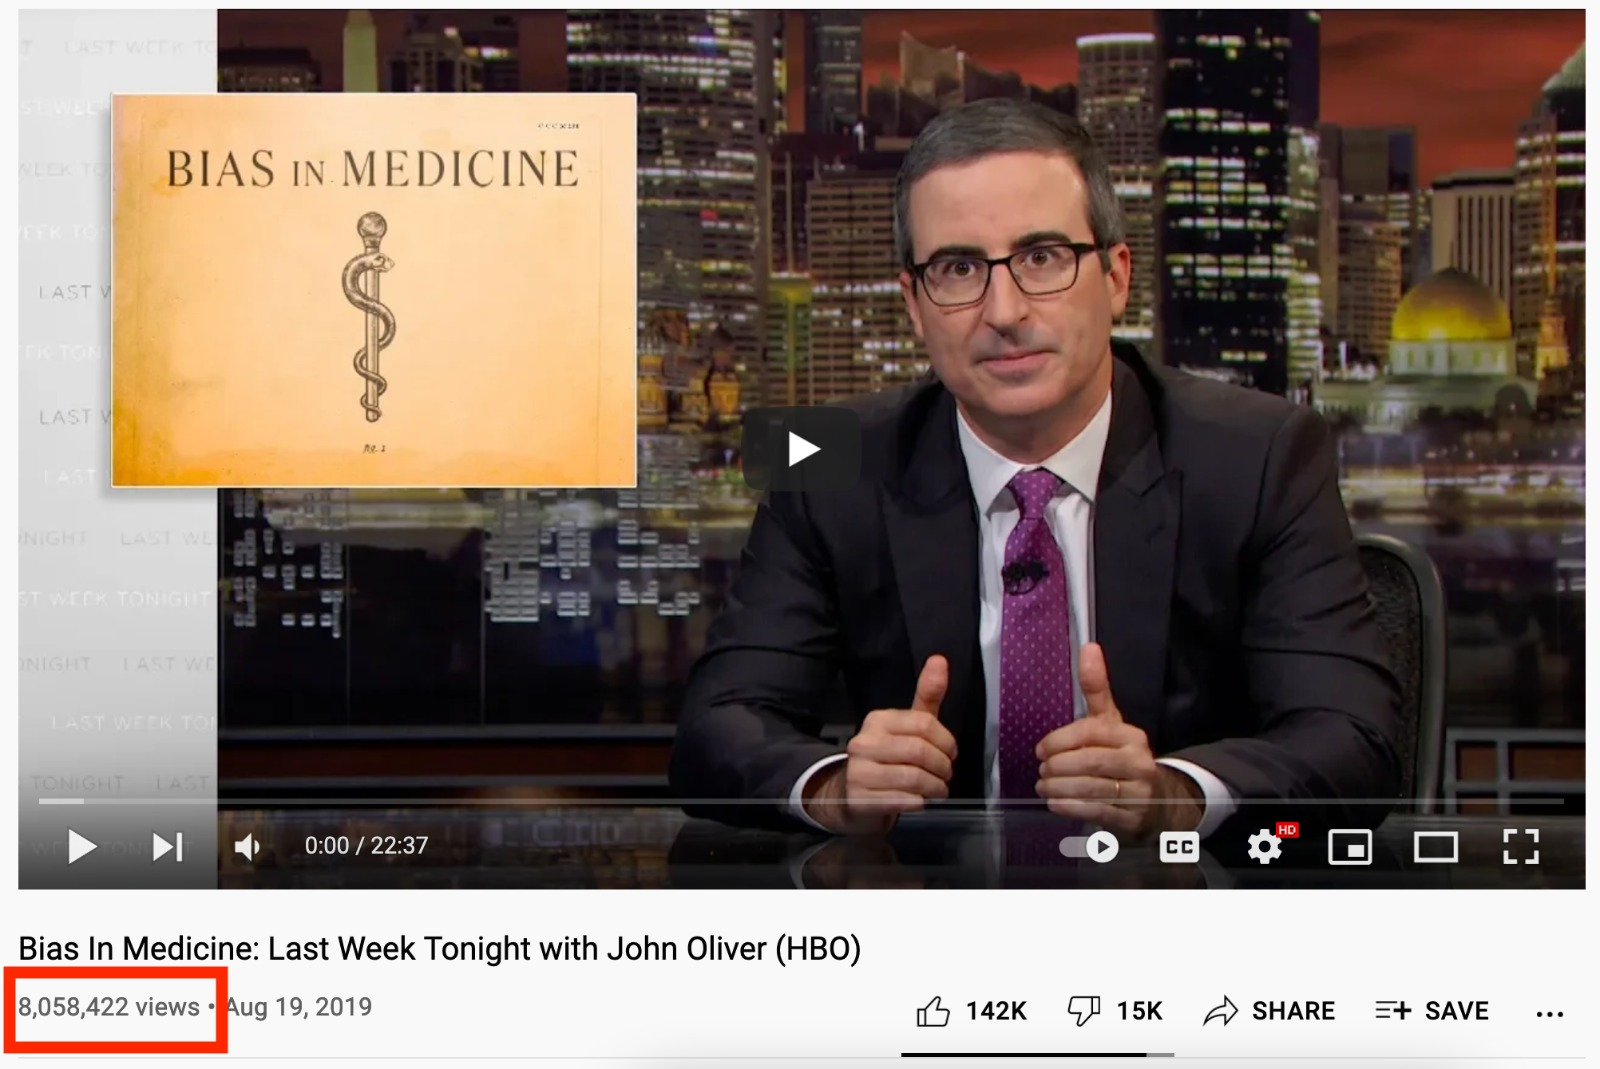
\includegraphics[width = \textwidth]{oliver.jpeg}}
	\end{figure}
\end{frame}




\begin{frame}[t,allowframebreaks]
\frametitle{References}
\bibliography{bibliography}
\end{frame}

\end{document}